% !TeX spellcheck = en_US
\begin{figure}[h] % also temporary
	\centering
	\begin{subfigure}[t]{0.5\textwidth}
		\centering
		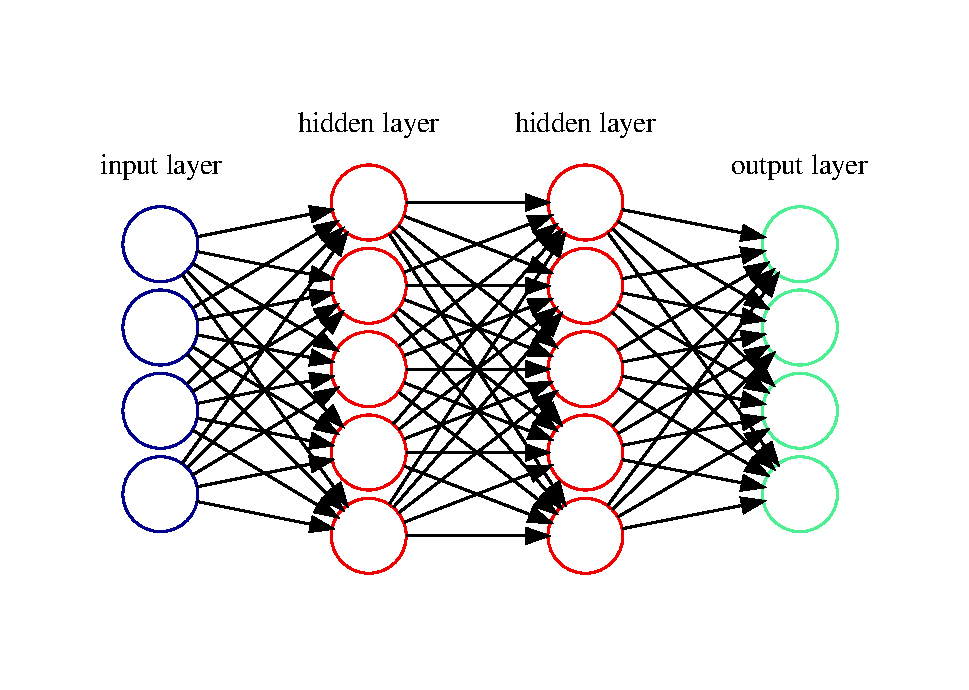
\includegraphics[width=\linewidth]{images/graphviz/general.pdf}
		\caption{An example for a neural network}
		\label{fig:neuralnetwork-general}
	\end{subfigure}%
	~ 
	\begin{subfigure}[t]{0.5\textwidth}
		\centering
		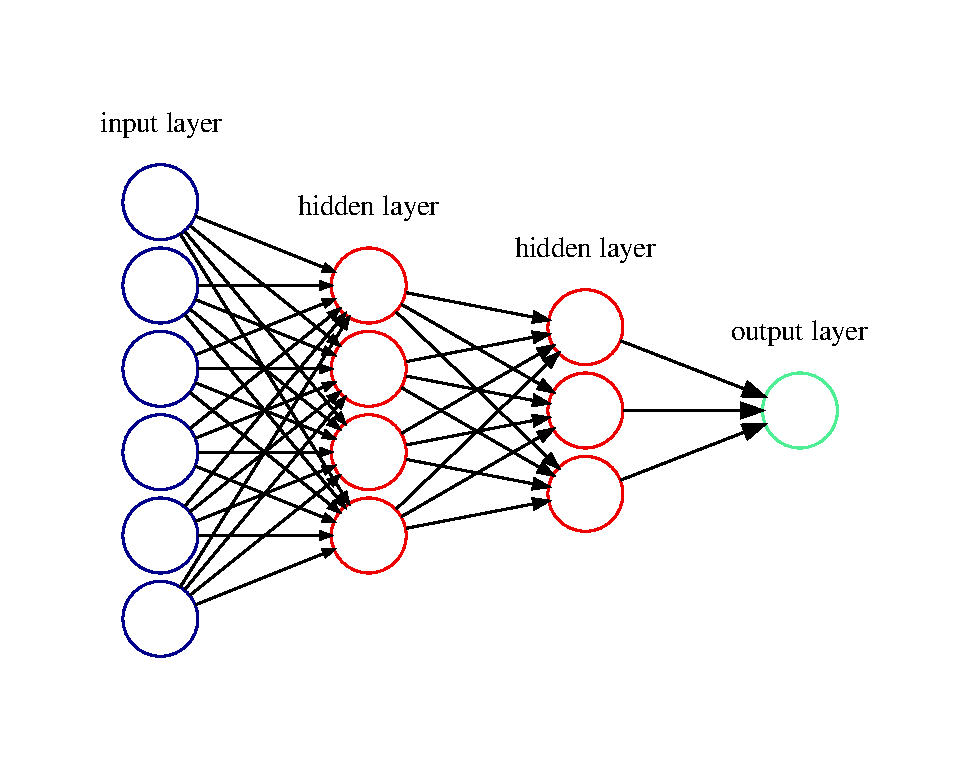
\includegraphics[width=\linewidth]{images/graphviz/graph.pdf}
		\caption{The network used for interpolation}
		\label{fig:neuralnetwork-graph}
	\end{subfigure}
	\caption{}
	
\end{figure}

\section{Artificial Neural Networks}

Another method that is good at taking pairs of input and output values and then able to predict output values for arbitrary input sets is using \textit{Artificial neural networks} (\texttt{ANNs}).

\subsection{Theory}

The idea behind artificial neural networks is trying to emulate the functionality of neurons by having nodes that are connected to each others. The weights $w$ of these connections are modified during the training to represent the training data and can then be used to predict new results for input values not seen in the training data.

Every neural network needs an input layer with as many nodes as input parameters and an output layer with a node for every output value. In between, there can be multiple hidden layers with an arbitrary number of nodes. (Figure \ref{fig:neuralnetwork-general})

If we first only consider a single neuron, then on every iteration it calculates the sum over all input values multiplied with their weight $w$. Afterwards an activation function $g$ is applied to the sum $z$ to get the prediction $\hat{y}$.

\begin{equation}
	z=\sum_{i}w_ix_i \qquad \hat{y}=g(z)
\end{equation}

The non-linear activation function allows the network to be able to approximate all types of functions instead of being just a linear function itself. Popular activation functions are the sigmoid function $\sigma(x)={\frac {1}{1+e^{-x}}}$ and the ReLU function (\textit{rectified linear unit}, $f(x)=\max(0,x)$).\footcite{NN-math}

After this first step (the \textit{feedforward}) is done, the weights can be modified by comparing the prediction with the real output (the \textit{backpropagation}). The function that describes the error between them is called the Loss function and one possible form is the mean squared error function:

\begin{equation}
	L(\hat{y},y)=\sum_{i}(\hat{y}_i-y_i)^2
\end{equation}

To update the weights, the derivative of the Loss function with respect to the weights is calculated and added to the existing weights.\footcite{NN-python}

\subsection{Implementation}

As building a neural network from scratch gets complex very quickly, it is easier to use \texttt{Keras}\footnote{\url{https://keras.io}} which provides easy to use high-level functions over the calculations provided by \texttt{TensorFlow}\footnote{\url{https://www.tensorflow.org/}}. To build our network, we only need to specify the structure of the layers, take our input and let the network train for 200 epochs (iterations of feedforward and backpropagation). 

The network needs six nodes in the input layer for the input parameters and one node in the output layer for the prediction. In between, are two layers with decreasing numbers of nodes as this seems to give the best results. (Figure \ref{fig:neuralnetwork-graph})

\begin{lstlisting}[language=Python,caption=The used model as Keras code,label=lst:model]
from keras import Sequential
from keras.layers import Dense

model = Sequential()
model.add(Dense(6, input_dim=6, activation='relu'))
model.add(Dense(4, kernel_initializer='normal', activation='relu'))
model.add(Dense(3, kernel_initializer='normal', activation='relu'))
model.add(Dense(1, kernel_initializer='normal', activation="sigmoid"))
model.compile(loss='mean_squared_error', optimizer='adam')

model.fit(x, Y, epochs=200, validation_data=(x_test, Y_test))

\end{lstlisting}

\subsection{Training}

To find the ideal parameters to use, the simulation data (excluding the data from Section \ref{sec:comparison}) is split into two groups: The complete original set of simulations and \SI{80}{\percent} of the new simulation set is used to train the neural network while the remaining \SI{20}{\percent} are used for validation. This means that after every epoch the loss function is not only calculated for the training data, but also for the separate validation data (Figure \ref{fig:loss_val}). Finally, the model with the lowest loss on the validation data set was chosen (Listing \ref{lst:model}).


\begin{figure}[h] % also temporary
	\centering
	\begin{subfigure}[t]{0.5\textwidth}
		\centering
		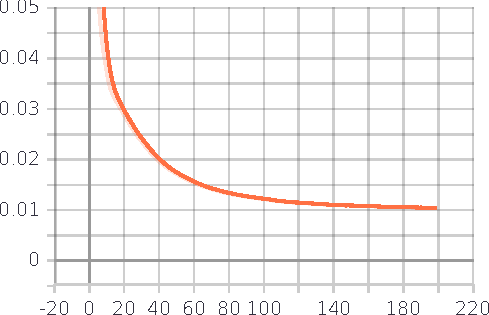
\includegraphics[width=\linewidth]{images/loss.pdf}
		\caption{loss function on the training data}
		\label{fig:loss}
	\end{subfigure}%
	~ 
	\begin{subfigure}[t]{0.5\textwidth}
		\centering
		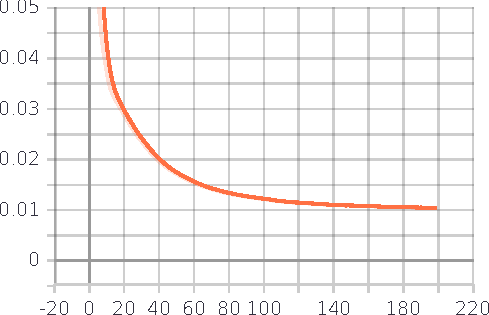
\includegraphics[width=\linewidth]{images/val_loss.pdf}
		\caption{loss function on the validation data}
		\label{fig:val_loss}
	\end{subfigure}
	\caption{During training the loss function (mean squared error) decreases with every epoch until it converges to a final value.}
	\label{fig:loss_val}
	
\end{figure}

After the training, the resulting model is saved in a small \texttt{HDF5} file which can be used to evaluate the model very quickly (about \SI{100}{\milli\second} for \num{10000} interpolations).


\subsection{Results}

Figure \ref{fig:nnresults} \todo{text}

\begin{figure}[h!] % also temporary
	\centering
	\begin{subfigure}[t]{0.5\textwidth}
		\centering
		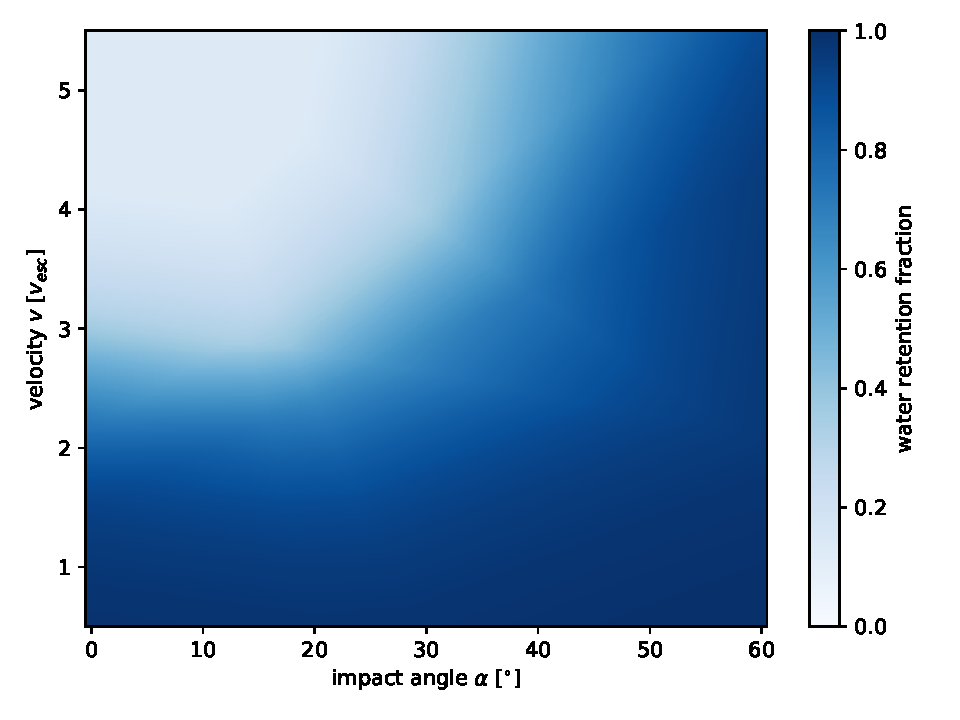
\includegraphics[width=\linewidth]{images/plots/nn1.pdf}
		\caption{$m_{total}=\num{e22}$, $\gamma=0.6$, $wt=wp=0.15$}
		\label{fig:nn1}
	\end{subfigure}%
	~ 
	\begin{subfigure}[t]{0.5\textwidth}
		\centering
		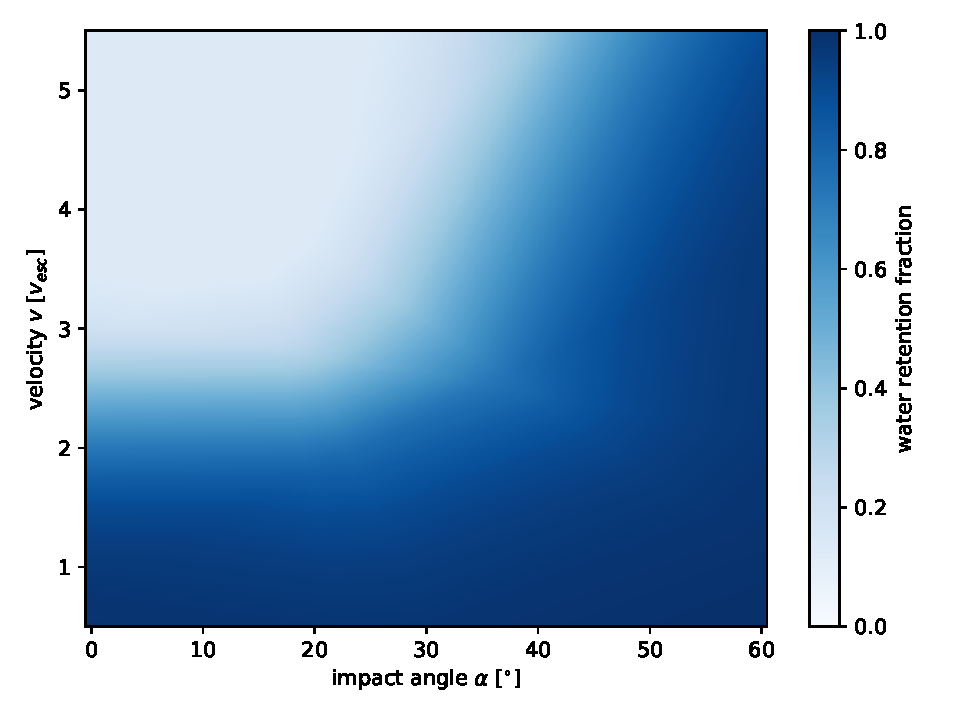
\includegraphics[width=\linewidth]{images/plots/nn2.pdf}
		\caption{$m_{total}=\num{e24}$, $\gamma=0.6$, $wt=wp=0.15$}
		\label{fig:nn2}
	\end{subfigure}
	\caption{Interpolation result using the trained neural network}
	\label{fig:nnresults}
\end{figure}
